\documentclass[conference]{IEEEtran}
\usepackage{graphicx}
\usepackage{booktabs}
\usepackage{amsmath}
\usepackage{url}
\usepackage[hidelinks]{hyperref}
\graphicspath{{../figures/}}
\title{Predicting Patient-Reported Drug Side-Effect Severity from Drug Reviews}
\author{\IEEEauthorblockN{Author One and Author Two}
\IEEEauthorblockA{Department and Institution\\Venue placeholder\\email@example.com}}
\begin{document}
\maketitle

\begin{abstract}
We re-evaluate a three-class classifier for patient-reported drug side-effect severity using the official UCI Drug Reviews (Druglib.com) split. The thesis pipeline is retained: spaCy lemmatization, TF--IDF text features, one-hot categorical features, balanced Random Forest, Logistic Regression, and support-vector classifiers tuned with three-fold GridSearchCV. Re-running the official 3,107-row training and 1,036-row test files gives accuracies of 0.729 (Logistic Regression), 0.737 (Random Forest), and 0.737 (SVC). We correct class-label reporting and ROC probability-column alignment, and report overlap and preprocessing-leakage diagnostics. The results are evidence about this small, self-reported dataset, not clinical validation.
\end{abstract}
\begin{IEEEkeywords}drug reviews, side-effect severity, text classification, TF--IDF, reproducibility\end{IEEEkeywords}

\section{Introduction}
The task is to predict the severity reported for a patient review, not to classify drugs themselves. Our contributions are: (1) a from-scratch rerun on the official UCI files; (2) faithful preservation of the thesis feature pipeline, models, and grids; (3) correction of label and ROC reporting defects; and (4) integrity and supplementary analyses whose numbers are saved in the repository.

\section{Related Work}
Drug-review sentiment and aspect analysis has been studied using cross-domain learning \cite{Grasser2018}. Our implementation uses established linear, tree, and kernel classifiers \cite{Breiman2001,Cortes1995} with sparse information-retrieval features \cite{Manning2008} and scikit-learn \cite{Pedregosa2011}.

\section{Dataset and Preprocessing}
We use Drug Reviews (Druglib.com), UCI dataset ID 461 \cite{Kallumadi2018}. The official files contain 3,107 training and 1,036 test rows. The five original labels are No, Mild, Moderate, Severe, and Extremely Severe; we bin them as No, Mild+Moderate, and Severe+Extremely Severe. Three review fields are concatenated, lower-cased, lemmatized with spaCy, and filtered for alphabetic non-stopword tokens. Missing review text is replaced with an empty string. Categorical variables are effectiveness, rating, condition, and urlDrugName.

\section{Methodology}
TF--IDF uses at most 7,500 unigram/bigram features with min\_df=5 and max\_df=0.95. One-hot encoded categorical features are concatenated to the sparse text matrix. Random Forest, Logistic Regression, and SVC use class\_weight=balanced, random\_state=42, and the thesis grids with cv=3. The vectorizer and encoder are fit once on the training split for the faithful headline reproduction.

\section{Experimental Setup}
The primary test metrics are accuracy and corrected macro precision, recall, and F1. ROC curves use a probability refit for SVC, matching the appendix, while probability columns are aligned to each estimator's classes. All values and figures are generated by scripts in the repository's `results/` and `figures/` directories.

\section{Results}
\begin{table}[t]
\caption{Official-split primary results.}
\centering\begin{tabular}{lccc}
\toprule Model & Accuracy & Macro P & Macro R/F1\\\midrule
Logistic Regression & 0.729 & 0.704 & 0.746/0.720\\
Random Forest & 0.737 & 0.711 & 0.744/0.719\\
SVC & 0.737 & 0.712 & 0.731/0.715\\
\bottomrule\end{tabular}\end{table}

The corrected one-vs-rest macro AUCs are 0.875, 0.873, and 0.875 for Logistic Regression, Random Forest, and SVC, respectively. Figure~\ref{fig:cm} shows the SVC confusion matrix in the explicit No/Mild/Severe order.
\begin{figure}[t]\centering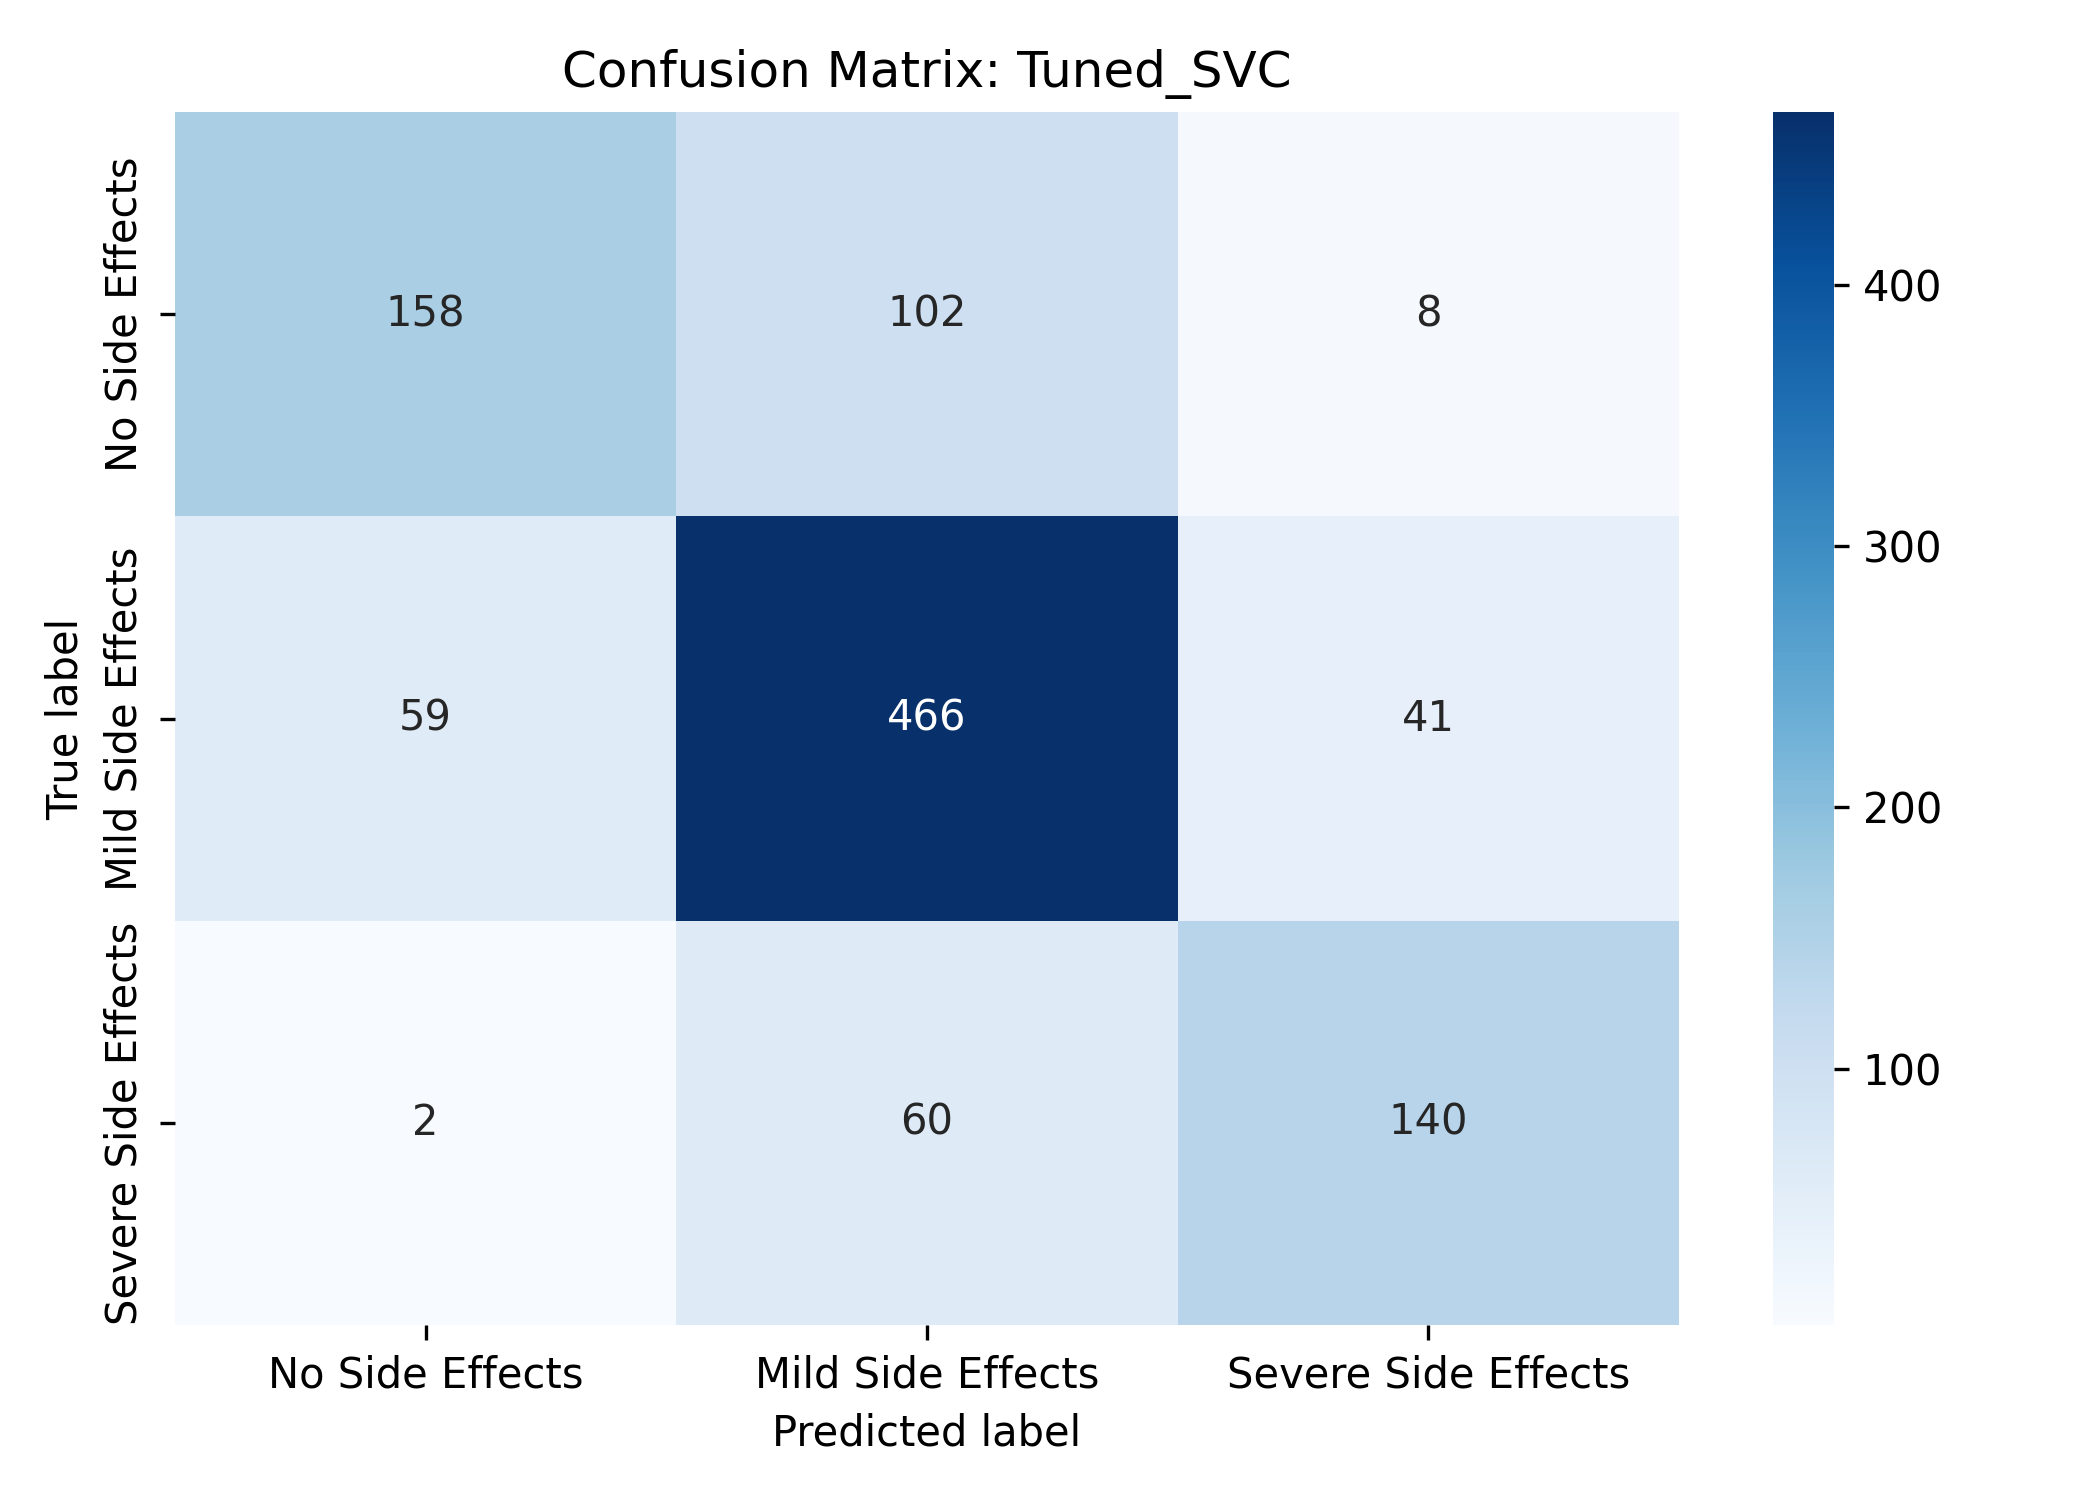
\includegraphics[width=0.95\columnwidth]{confusion_matrix_corrected_Tuned_SVC.png}\caption{Corrected SVC confusion matrix on the official 1,036-row test split.}\label{fig:cm}\end{figure}

\subsection{Integrity findings}
The thesis matrices sum to 1,200 rows and therefore cannot be direct outputs from the official 1,036-row test file. We find 16 exact combined-review overlaps and 20 near-duplicate training/test texts. The appendix fits TF--IDF and one-hot encoding before cross-validation, so its CV estimates are not fold-contained. These findings are reported rather than silently used to replace the primary result.

\subsection{Supplementary analyses}
With feature fitting inside stratified five-fold pipelines, mean accuracy is 0.702 (LR), 0.709 (RF), and 0.718 (SVC); corresponding macro-F1 means are 0.697, 0.694, and 0.702. Bootstrap 95\% accuracy intervals are [0.701,0.756], [0.711,0.763], and [0.709,0.764]. McNemar's exact test comparing SVC and RF is uninformative here: each model is uniquely correct on 84 cases (two-sided p=1.0). In the ablation, text-plus-categorical features outperform text-only and categorical-only settings for all three models.

\section{Discussion and Limitations}
The official split does not reproduce the thesis's 0.87--0.93 accuracy range. The discrepancy is not corrected by tuning. The label is self-reported and the sideEffectsReview text is close to the target definition; class weights address imbalance but do not remove label noise. The data are small, overlap exists, preprocessing is not fold-contained in the headline protocol, and no clinical or regulatory validation is claimed.

\section{Conclusion}
A transparent rerun preserves the undergraduate design while correcting two reporting defects and separating official results from thesis-reported values. The repository and Kaggle notebook provide executable evidence for further author decisions, including whether the original `download.csv` can be supplied for forensic comparison.

\bibliographystyle{IEEEtran}
\bibliography{refs}
\end{document}
